\section{Methodology}
% Description of your proposed methodology or approach
In this section, we display how effective image preprocessing and our docking procedure collectively lead to a plausible method to train our model without manual labeling, which would be required, for our case, in real-world applications. Our methodology includes data collection, data preprocessing, model training, inference, server integration, evaluation, and experimental setup.

\subsection{Data Collection}
We collect training data using a simulated environment created in a game engine \citep{hoster2024usinggameenginesmachine}. Our game engine of choice is Godot, a free and open source game engine. The environment consists of a robot, a data camera, the alignment target (target 1) and the docking station (target 2). The data camera is scripted so that it captures images of the environment from various angles. The target that the data camera focuses on during the data gathering process can either be the alignment target or the docking station. What is important is that, in our data preprocessing, we exclude images that don't have their respective target in them, as explained in the next section.

The data camera is not randomly moving, and then taking a picture. Rather, it moves right to left in a predefined amount of steps. At each step, the data camera looks at our target, and rotates a predefined angle horizontally. This is because each step has its own number of what we call rotational images, which are images that are taken at the position of the step, but horizontally rotated slightly each time. Once the data camera has reached the end of the row moving left, we can move forward to the next row, and repeat the process. We do this until we are close enough to the dock.
\begin{figure}
    \centering
    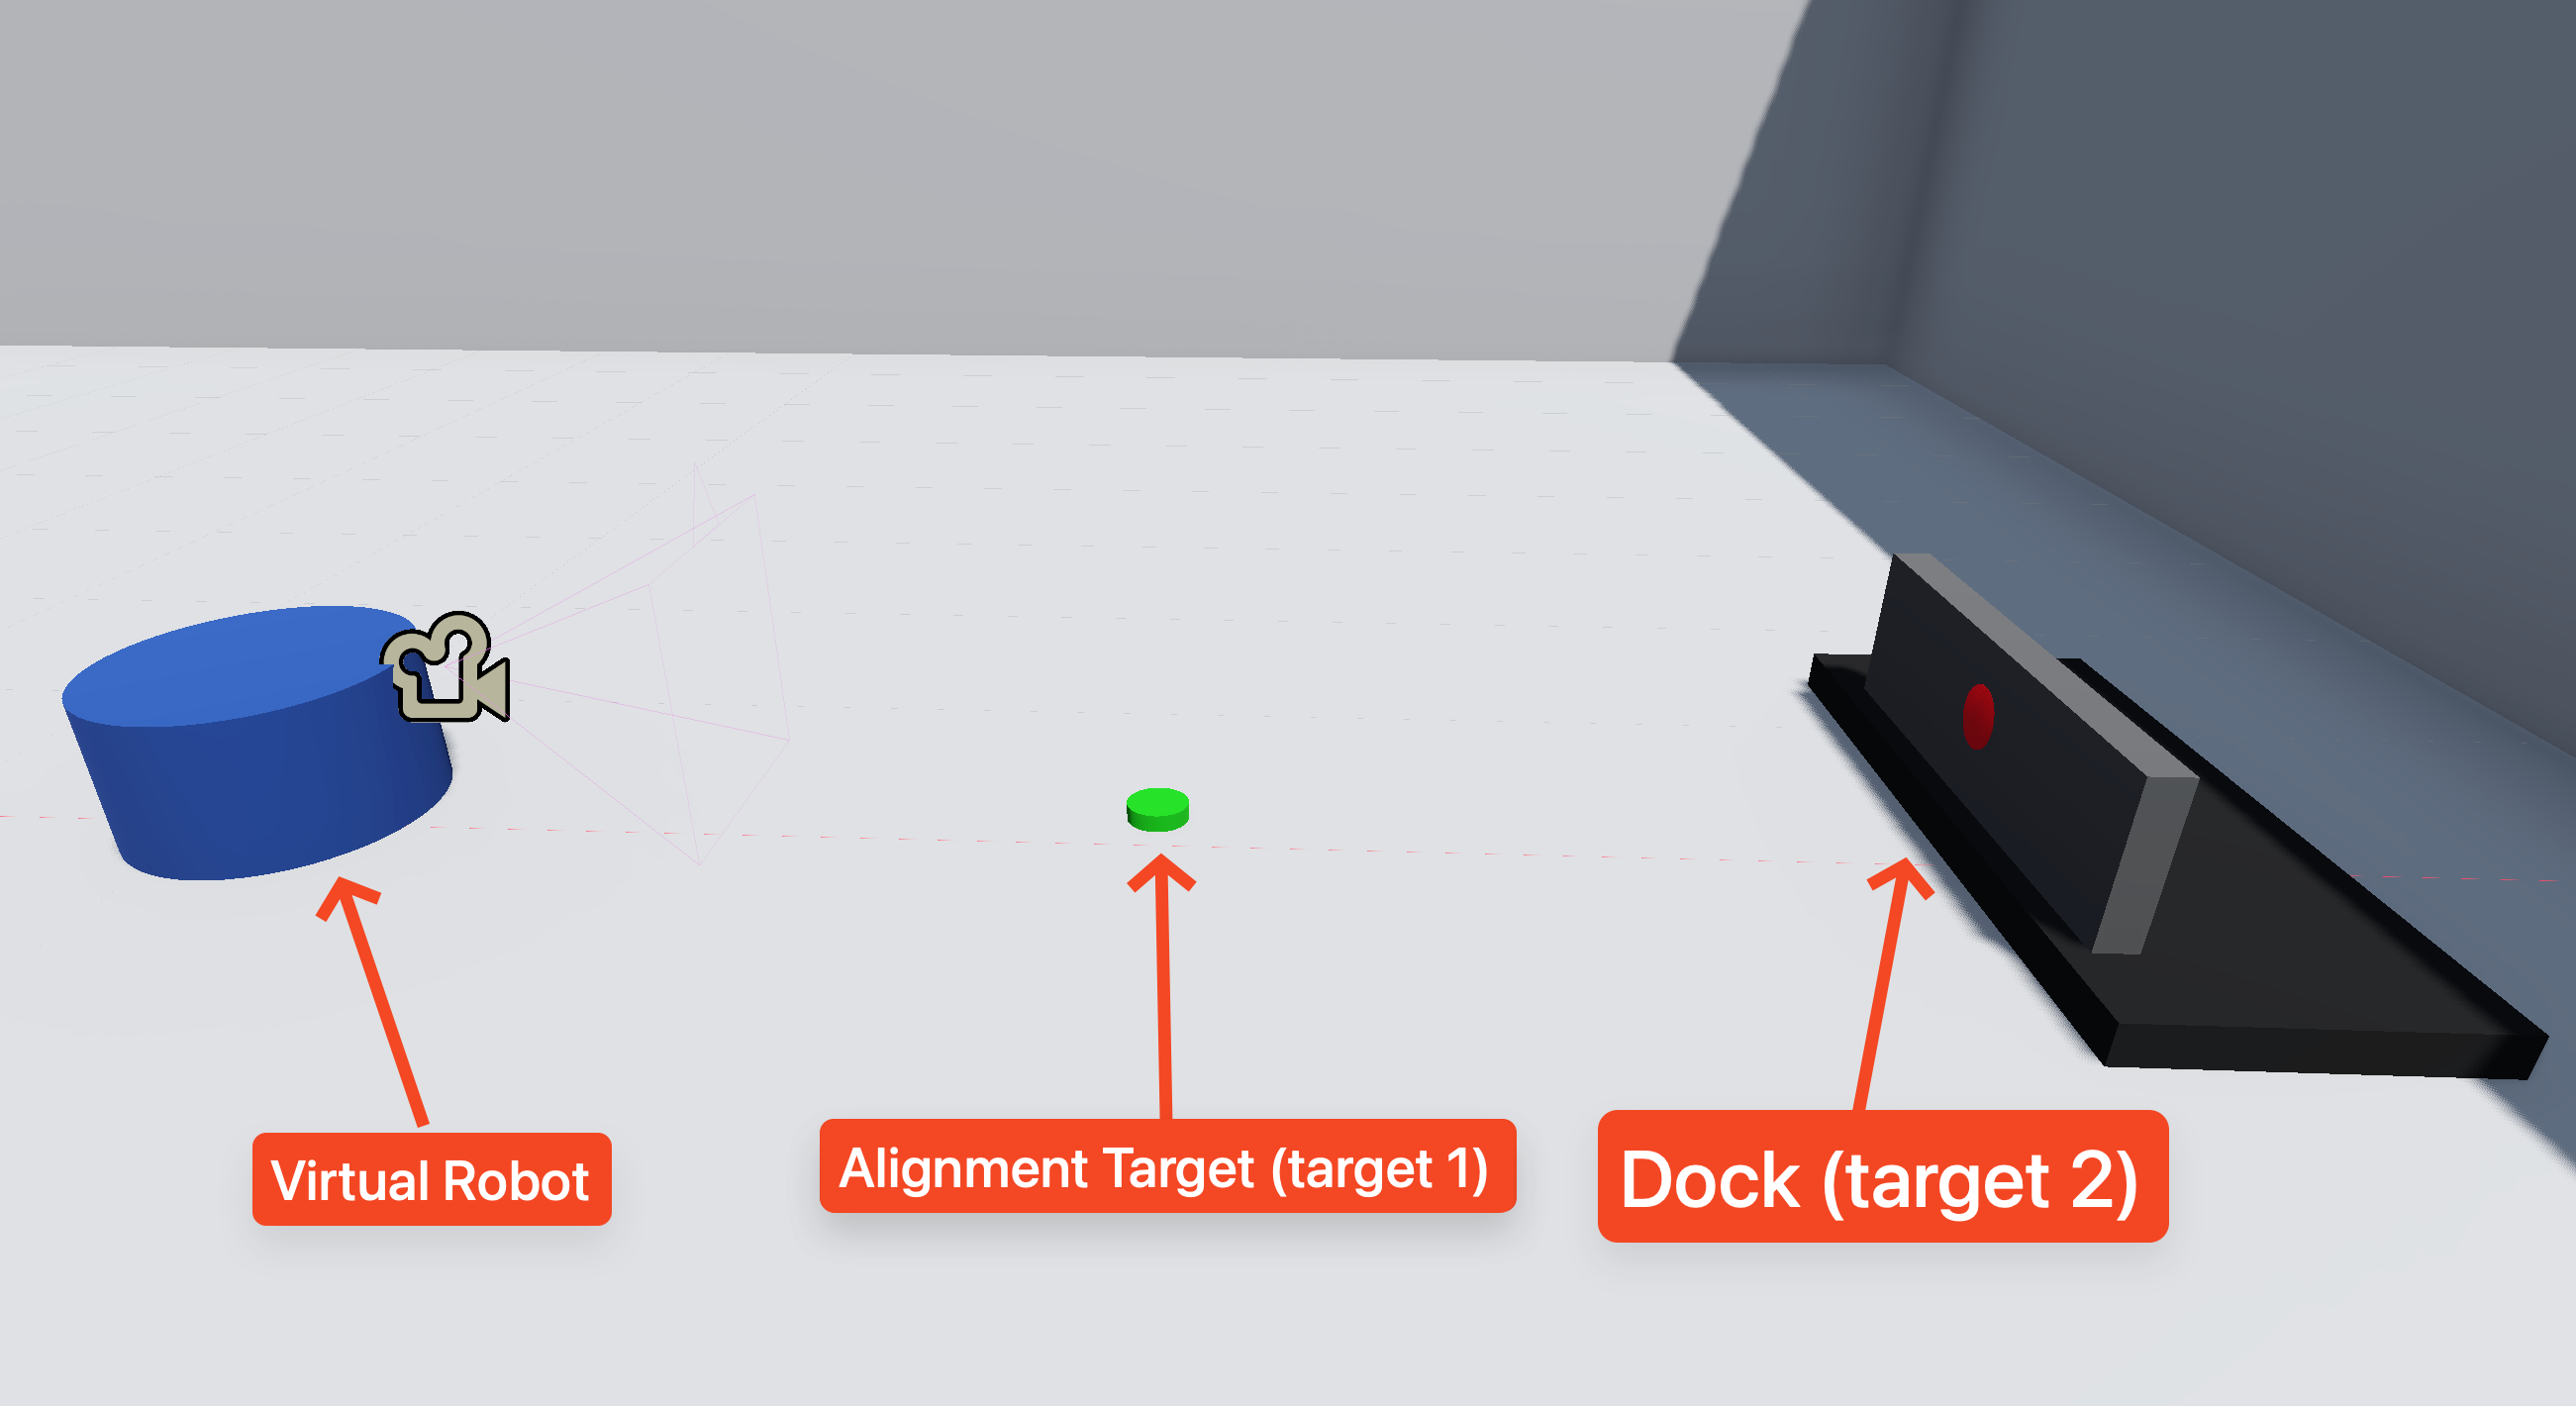
\includegraphics[width=\linewidth]{figures/src/virtual_world.png}
    \caption{
	    \textbf{Virtual world \& Labels} In our virtual world, we make targets 1 and 2 distinguishable from their surrounding environment by giving them a unique color.
    }
    \label{fig:virtual world}
\end{figure}


The reason we want to collect our data this way is because we want to make our data inclusive. With randomization, we don't know for sure if there will be images that are extremely similar, and we don't know if each angle is represented fairly. The diagram below shows what the data camera movement looks like from a bird's eye view.
\begin{figure}[htbp]
    \centering
    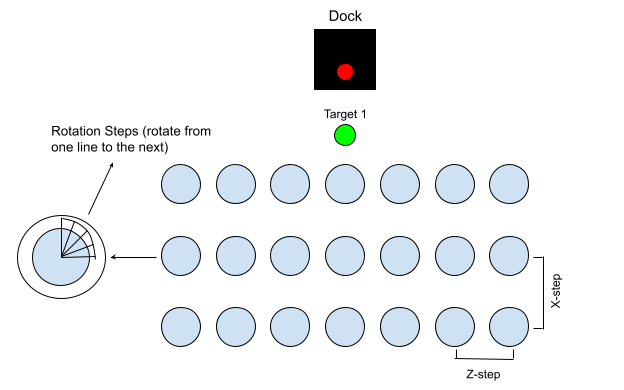
\includegraphics[width=0.9\columnwidth]{figures/src/data_camera_movement_algo.png}
    \caption{
	    \textbf{Data Camera Movement Procedure} Our data camera moves in z-steps and x-steps, with rotations for each z-step. We obtain an image with each rotation step.
    }
    \label{fig:data_camera_movement_algo}
\end{figure}


\subsection{Data Preprocessing}
We preprocess the collected images in order to have a dataset of images and their corresponding target values. In order to do this, we use OpenCV to detect the targets. This is really only a viable option due to the fact that we chose unique colors for our targets that aren't present anywhere else in the virtual world. In real life, contour detection like this wouldn't work, and we would need to manually label where the targets are.

Contour detection returns a list of coordinates that outline a target. We, however, only want one coordinate. We can achieve this by approximating the center of the target, which can be done by taking the mean of both the \(x\) and the \(y\) values of the contour coordinates list:

\[
	\bar{x} = \frac{1}{n}\sum_{i=1}^{n} x_i ~\text{,} ~\bar{y} = \frac{1}{n}\sum_{i=1}^{n} y_i
\]
\begin{figure}[H]
    \centering
    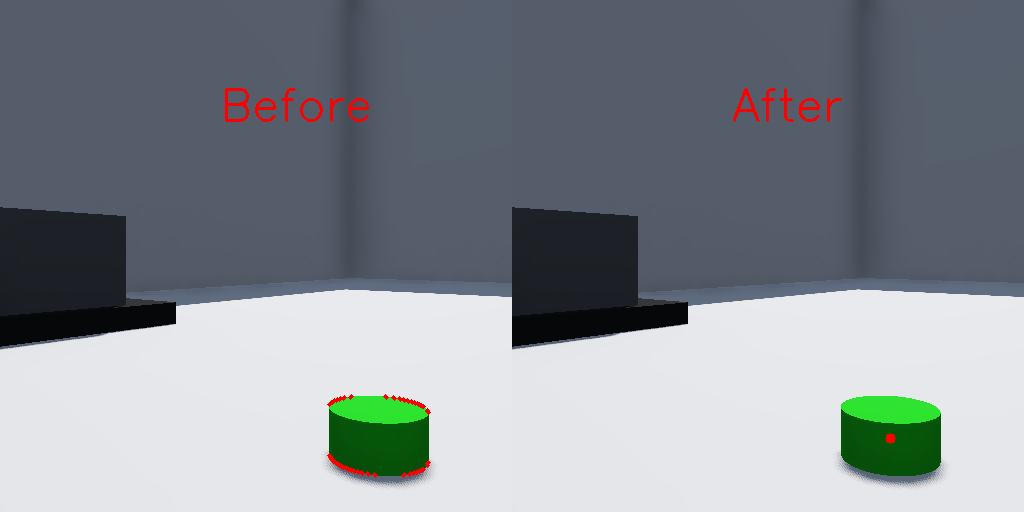
\includegraphics[width=0.9\columnwidth]{figures/src/contour_and_average.png}
    \caption{
	    \textbf{Averaging contour points} By averaging contour points, we have one point of reference for the target object.
    }
    \label{fig:contour_and_average}
\end{figure}


Where \(n\) is the number of points in the contour, and \(x_i\) and \(y_i\) are the \(x\) and \(y\) parts of each point in the contour, respectively. This gives us a single coordinate for each target, which we can then use as our target value for training. Due to our images being 512x512 pixels, the coordinates are in range from 0 to 512 (for both \(x\) and \(y\)). This means that the coordinates are then normalized from 0 to 512 to 0-1 by dividing the coordinates by 512. This way, model training and inference becomes easier and more efficient, as we are not dealing with large numbers \citep{SINGH2020105524}. Of course, when it comes to inferencing, we then multiply the model's outputs by 512 to get the actual coordinate values. 

Our data is then sorted into two sets of data, one set specifically for the alignment target, and one specifically for the docking station. The reason we do this is because our custom models are not trained the same way YOLO models are trained, meaning we can't know for sure if the object is actually in frame. So, if one target is in an image, it doesn't necessarily mean that the other one is as well. The two sets of data share images, but one set may have more or less images than the other. This is because at some angles, one target may be visible while the other is not. In our case, the set of data that has more images is the one where we focused the target on during data gathering in the Godot game engine, which was target 1 (the green target). 

\begin{figure}[H]
    \centering
    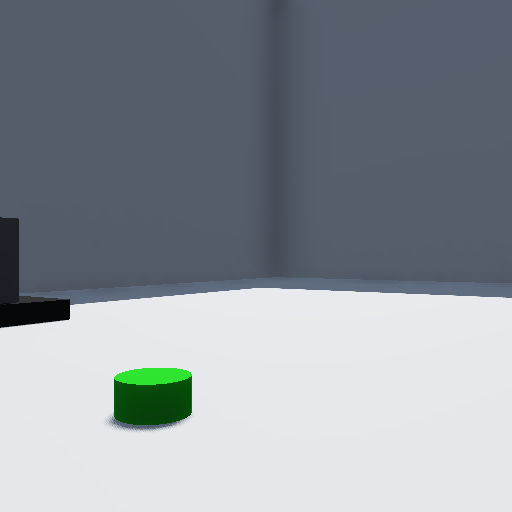
\includegraphics[width=0.7\columnwidth]{figures/src/target_1_but_not_target_2.png}
    \caption{
	    \textbf{Differing Image Amounts} An example of an image that includes target 1 (alignment target) but not the red part of target 2 (dock). 
    }
    \label{fig:target_1_but_not_target_2}
\end{figure}


This sorting of data for each model is done through OpenCV. If contour detection is not present for one of the targets, the image is not included in the dataset for the target not found. This applies to both targets in the same function, meaning, if no targets are found, the image is essentially discarded. Again, using OpenCV for these operations is highly possible because we are in a virtual environment where the colors of the targets are unique to themselves.

The sorting of data for the two separate models also means that each model may be performed differently. However, in our data collection, the difference in image amount was around 1,148, meaning we had 1,148 more images for the target we focused on. This is not a concerning difference, and we can still train the models in very similar ways. The only difference is that the model that has less images may have a lower accuracy, which is where our custom data augmentation comes in.


\subsection{Model Training}
Near the end of this paper, we describe how our methodology can be implemented using a single YOLO model for object detection and prediction, all in one package. The reason why we have initially developed our project with custom models is because we have more flexibility regarding the architecture and performance of the models. By implementing the models using PyTorch, we can make lower level modifications to essentially see what the most conservative model is that can still perform well. This is important because we want to make sure that our model is as lightweight as possible while delivering adequate results. We don't want to have a model that is too heavy, because it will be running on a robot that has limited computational power.

Our training process is quite standard and is as follows:
\begin{enumerate}
    \item Load and preprocess the images using the `transforms` module from torchvision.
    \item Define the custom dataset class `TargetsDataset` to handle the input data.
    \item Instantiate the model, loss function (L1 Loss), and optimizer (Adam).
    \item Train the model over multiple epochs, applying custom image augmentation techniques to improve generalization.
\end{enumerate}

The first, second, and third steps in the list above are all standard ways to train a PyTorch model, or any basic deep learning model like the one we are creating. For the fourth step, the reason we need to apply custom image augmentation is because of coordinate predictions on the image. If we use the built-in method of image augmentation that PyTorch provides, the coordinates of the data will be off. The image is being transformed, but the coordinates are not. 

In order to solve this, we implement our own vertical flip augmentation, which returns the transformed image and the transformed coordinates. This way, the model can learn to predict the correct coordinates, even if the image is flipped. The reason we only need to implement a vertical flip is because, if we also implemented the horizontal flip, the data would have very similar looking images, as the flipped images would be almost identical to the images taken on the other side of the robot during data gathering.

\subsection{Inference}
% In this section we talk about how we can use both models in order to guide the robot and make actions.
For inference, we use the trained models to output the values necessary to determine the next action, all based on a single input frame. When targeting either one of the targets during the docking procedure, we use some mathematical boundaries to determine the action the robot should take.

There are three areas the predicted coordinates can be in which are listed below. Each area corresponds to an action, which is referenced to in the server integration section:

\begin{enumerate}
	\item The coordinates are outside the boundaries of what is considered centered with the target. In this case, the robot should turn either left or right, depending on the side the coordinates are on.
	\item The coordinates are inside the boundaries of what is considered centered with the target. In this case, the robot should move forward.
	\item The coordinates are inside the boundaries of what is considered centered with the target, under a certain threshold. This is a special case where the robot moves forward a fixed amount, and only applies to the alignment target (target 1).
\end{enumerate}

\textbf{Here we add a diagram showing the three areas on an example image}


For the third case, which only applies to the alignment target (target 1) the robot has reached the target if the predicted coordinates are within the boundaries for the robot to be considered centered with the target, but are under a certain threshold. So, if the predicted coordinates are within a bottom center area of the image, the robot should move forward a fixed amount. The reason we move forward a fixed amount is because we want to be above the alignment target in order to ensure we are then centered with the docking station (target 2).

\subsection{Server Integration}
To facilitate real-time predictions, we can integrate the inference script with a Flask server. The server receives images via POST requests, runs the inference, and returns the next action the virtual robot should take. The actions possible are shown in the table below: 

\begin{table}[H]
	\centering
	\begin{tabular}{|c|c|}
		\hline
		Action & Description \\ \hline
		0      & Turn left   \\ \hline
		1      & Turn right  \\ \hline
		2      & Move forward \\ \hline
		3      & Move forward fixed amount \\ \hline
	\end{tabular}
\end{table}

We use a Flask server so that GDScript can communicate with the Python script. The Python script is running the server, and the GDScript is sending the encoded images to it. The server then sends back the action the robot should take.

Again, we incorporate such a process in the first place because we are dealing with a virtual world that needs to communicate with Python, which is separate. In reality, however, we would have the robot do everything on its own, without the need for a server. Everything would be incorporated between scripts rather than between a separate server and a script.

\subsection{Evaluation}
\textbf{Todo: Determine if this section is necessary.}
We evaluate the performance of our model using various metrics, including accuracy and loss values. The evaluation scripts are included in [tests/tests.py](tests/tests.py), which contain unit tests to ensure the correctness and robustness of our data processing and model training pipelines.

\subsection{Experimental Setup}
The experimental setup we have presented so far is about the virtual world and the docking procedure. However, we also need to consider the hardware requirements for the training of our models, and what it took for us to get them running.

The models were trained on an M1 Macbook Air with 16 GB of RAM. The training process took around 40 minutes for each model using the CPU, and around 15-20 minutes using the GPU through PyTorch's MPS backend. The models trained using the hardware mentioned were the ones used to make our conclusions. Our purpose of training the models on a Macbook Air, or any other computational device without expensive hardware, is to show that our methodology is robust and that our inference requires very little computational power.

\subsection{Conclusion}
The methods used to get synthetic data were simple yet effective. We used the Godot game engine, which runs efficiently on low-power hardware (such as an arm chip MacBook), and we used OpenCV to obtain ground truth data. Using this data, we sorted it and trained our custom models, of which we had low-level control of to determine sufficient proficiency at an efficient computational cost. Our methodologies can be expanded in a similar manner to real-world applications and images, with the only difference being that we would need to manually gather and label the images instead of having them automatically taken by Godot and labeled using OpenCV.
